
\documentclass[10pt,a4paper]{article}

%%%%%%%%%%%%%%%%%%%%%%%%%%%%%%%%%%%%%%%%%%%%%%%%%%%%%%%%
%
% Packages and Theorem Environments

\usepackage{graphicx}
\usepackage{psfrag}
\usepackage{epsf}
\usepackage{amsmath,amsfonts,amssymb,latexsym}
\usepackage{enumitem}
\usepackage{algorithmic}
\usepackage{algorithm}
\usepackage[width=160mm,height=240mm,left=35mm,foot=10mm]{geometry}
\usepackage{xcolor}
\usepackage{url}
\usepackage{hyperref}
\usepackage{tikz}



\renewcommand{\theequation}{\thesection.\arabic{equation}}
\newcommand{\makeTiny}[1]{{\tiny #1}}
\newcommand{\work}{\tiny}
\newcommand{\ignore}[1]{}
\newcommand{\startClaims}{\setcounter{claim}{0}}
\newtheorem{theorem}{Theorem}[section]
\newtheorem{corollary}[theorem]{Corollary}
\newtheorem{lemma}[theorem]{Lemma}
\newtheorem{proposition}[theorem]{Proposition}
\newtheorem{conjecture}[theorem]{Conjecture}
\newtheorem{problem}[theorem]{Problem}
\newtheorem{question}[theorem]{Question}
\newtheorem{definition}[theorem]{Definition}
\newtheorem{task}[theorem]{Task}
\newtheorem{claim}{Claim}
\newtheorem{remark}[theorem]{Remark}
\newtheorem{observation}[theorem]{Observation}

\graphicspath{hw3}



\title{MATH 351--004 -- Assignment \#$3$\\
}

\author{Alex Iacob\\
ai9388}

\date{September 16, 2021}


%%%%%%%%%%%%%%%%%%%%%%%%%%%%%%%%%%%%%%%%%%%%%%%%%%%%%%%%
%
% Author's definitions


\newcommand{\NN}{\mathbb N}
\newcommand{\ZZ}{\mathbb Z}
\newcommand{\QQ}{\mathbb Q}
\newcommand{\RR}{\mathbb R}

\newcommand{\BB}{\mathcal B}
\newcommand{\ZT}{\mathcal Z}

\newcommand{\Cl}{\operatorname{Cl}}
\newcommand{\Bd}{\operatorname{Bd}}
\newcommand{\row}{\operatorname{row}}
\newcommand{\col}{\operatorname{col}}
\newcommand{\Span}{\operatorname{span}}
\newcommand{\convhull}{\operatorname{conv.hull}}
\newcommand{\tr}{\operatorname{tr}}

\newcommand{\diam}{\operatorname{diam}}

\begin{document}

\maketitle

\subsection*{Problem 1 - For which integers $x$ ($0 \leq x \leq 7$), if any, is the sequence \\ $s$ = 7, 6, 5, 4, 3, 2, 1, x graphical?)}
Using Corollary 2.3, we know that every graph must have an even number of odd vertices, currently in s, there are 4 and adding another odd vertex would make the number odd, which we cannot have, therefore $x$ must be even.
\newline
Using Theorem 2.10:\\
\newline
x = 0\\
$s$ = 7, 6, 5, 4, 3, 2, 1, $0$\\
$s\prime$ = 5, 4, 3, 2, 1, 0, -1\\
Not graphical because there exists a negative number in $s\prime$. \\
\newline
x = 2\\
$s$ = 7, 6, 5, 4, 3, 2, 1, $2$\\
$s$ = 7, 6, 5, 4, 3, 2, 2, 1\\
$s\prime$ = 5, 4, 3, 2, 1, 1, 0\\
$s\prime\prime$ = 3, 2, 1, 0, 0, 0\\
$s\prime\prime\prime$ = 1, 0, 0, 0, -1\\
Not graphical because there exists a negative number in $s\prime\prime\prime$. \\
\newline
x = 4\\
$s$ = 7, 6, 5, 4, 3, 2, 1, $4$\\
$s$ = 7, 6, 5, 4, 4, 3, 2, 1\\
$s\prime$ = 5, 4, 3, 3, 2, 1, 0\\
$s\prime\prime$ = 3, 2, 2, 1, 0, 0\\
$s\prime\prime\prime$ = 1, 1, 0, 0, 0\\
Graphical because $s\prime\prime\prime$ is just 5 points with an edge between two vertices\\
\newline
x = 6\\
$s$ = 7, 6, 5, 4, 3, 2, 1, $6$\\
$s$ = 7, 6, 6, 5, 4, 3, 2, 1\\
$s\prime$ = 5, 5, 4, 3, 2, 1, 0\\
$s\prime\prime$ = 4, 3, 2, 1, 0, 0\\
$s\prime\prime\prime$ = 2, 1, 0, 0, -1\\
Not graphical because there exists a negative number in $s\prime\prime\prime$. \\

\subsection*{\newpage Problem 2 - Which pairs in Figure 3.12 are isomorphic? Explain your answer.}
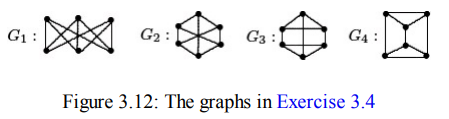
\includegraphics[width = 7cm]{fig312}

Two graphs, $G$ and $H$, can be labeled as isomorphic if there exists a correspondence between $V(G)$ and $V(H)$ such that 
$uv \in E(G) iff \phi(u)\phi(v) \in E(H)$. \\

Graph $G_{3}$ is isomorphic to $G_{4}$.\\
Graph $G_{1}$ is isomorphic to $G_{2}$.\\

Labeling these graphs' vertices in such way allows their structures to be the same.

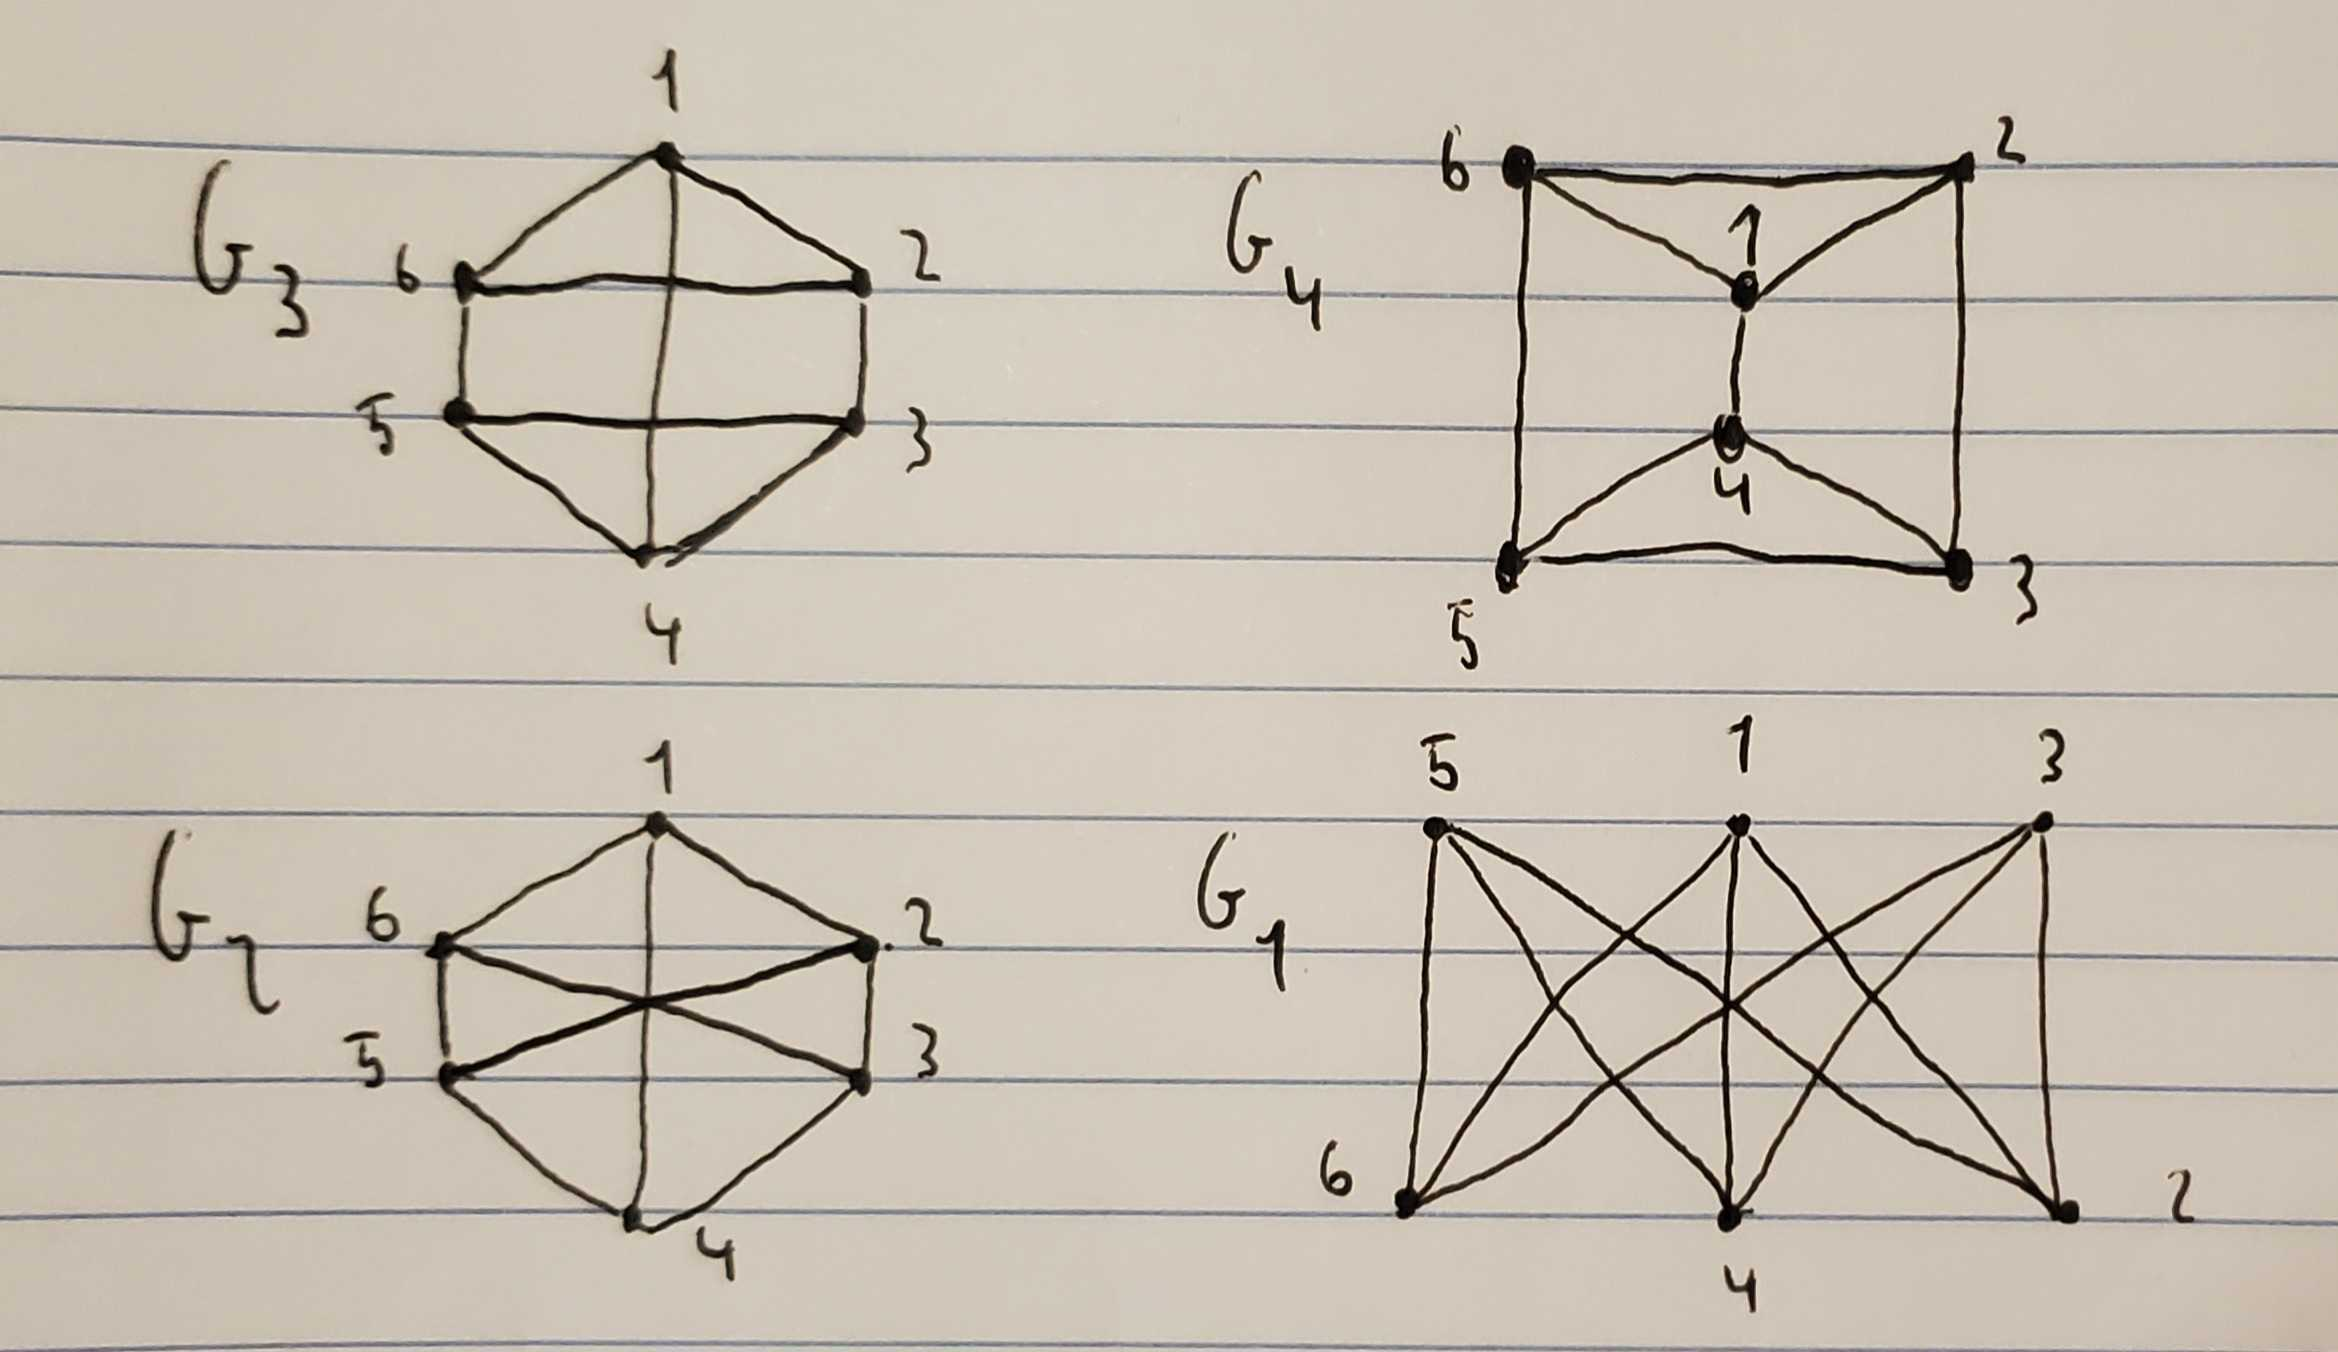
\includegraphics[width = 7cm]{problem2}

\subsection*{Problem 3 - How many (non-isomorphic) graphs have the degree sequence $s$: 6, 6, 6, 6, 6, 6, 6, 6, 6. (Nine 6's)}
Using Theorem 3.1, we can describe this graph's degree sequence as $s^{c}$: 2, 2, 2, 2, 2, 2, 2, 2, 2. \\
There are 4 general types of graphs that fall under this degree sequence, which are shown below. 
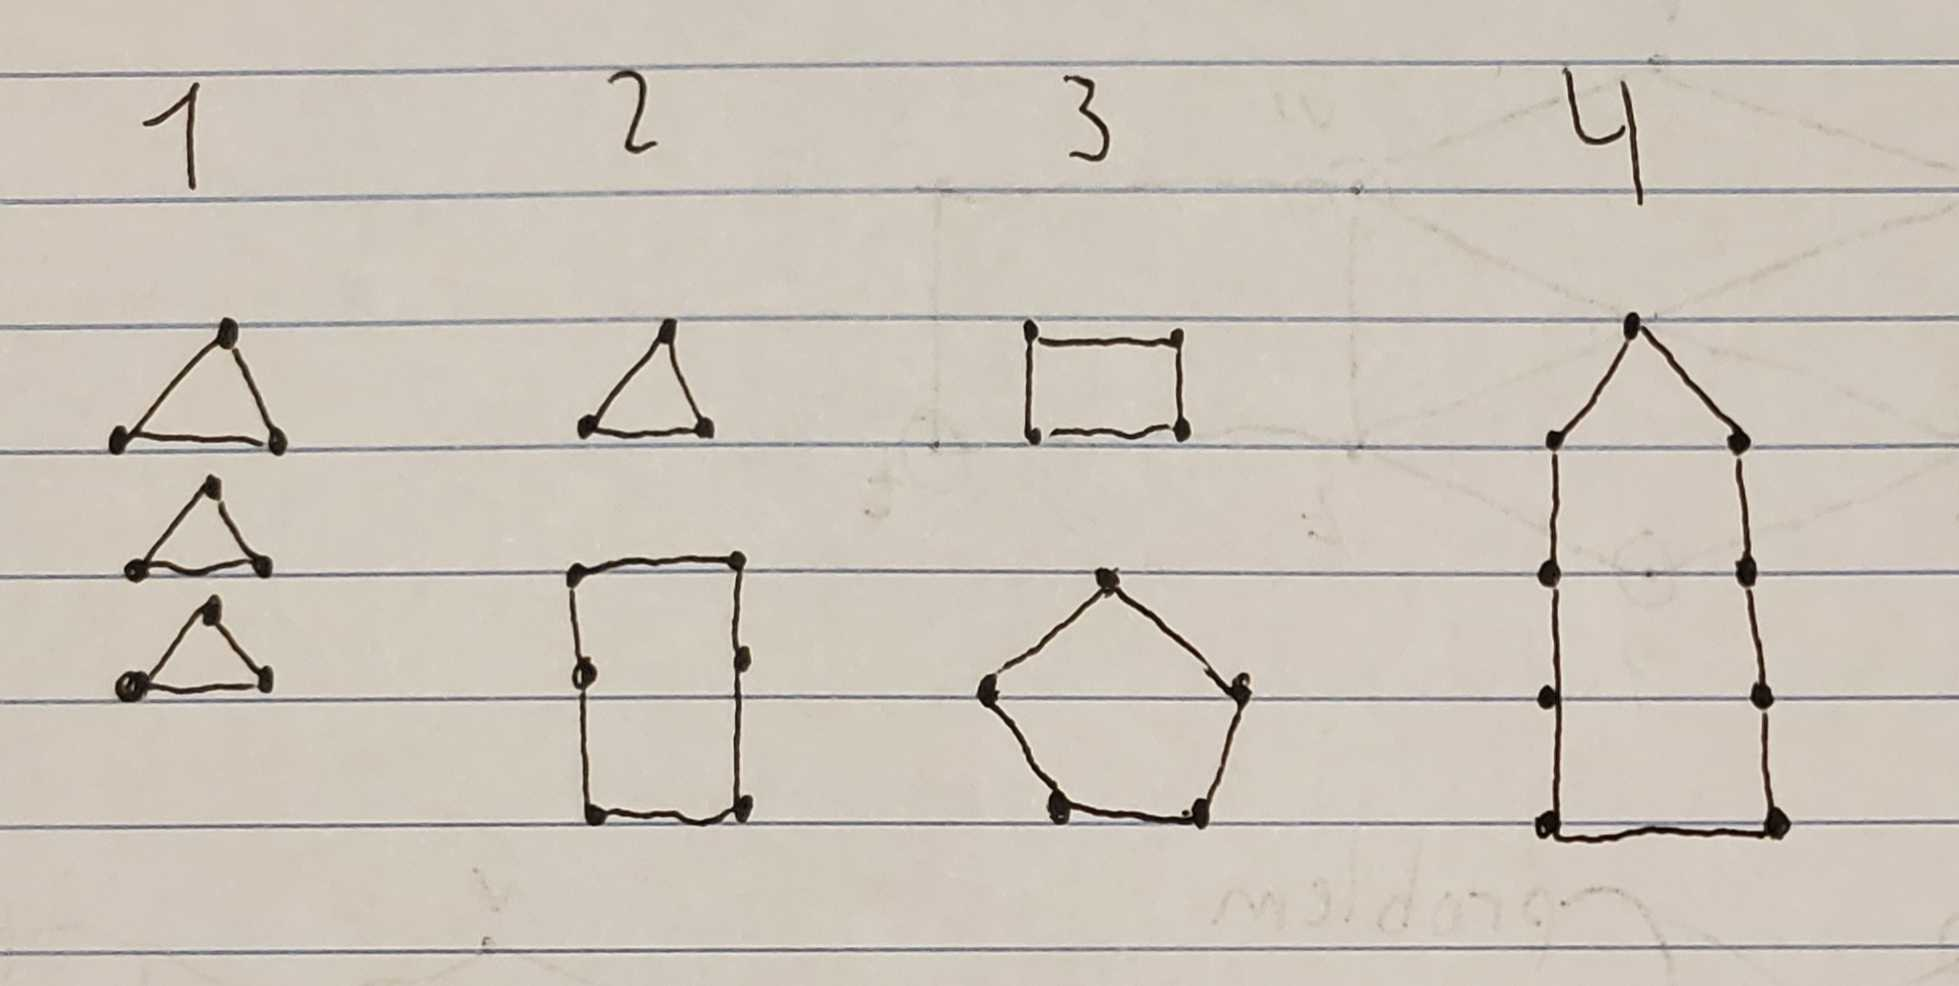
\includegraphics[width = 7cm]{problem3}

\subsection*{\newpage Problem 4 - For the deck $D$ of cards given in Figure 3.42, where card $i$ contains the subgraph $G_{i} = G \ v_{i}, v_{i} \in V(G)$, for some graph $G$, answer the following with explanation.}


$(a)$ What is the order $n$ of $G$?\\ The order is 7.\\
$(b)$ What is the size $m$ of $G$?\\ The size is 8.\\
$(c)$ What are the degrees of vertices in $G$?\\ $s$ = 3, 3, 2, 2, 2, 2, 2 \\
$(d)$ Is $G$ connected?\\ $G$ is connected.\\
$(e)$ What are the solutions of $D$\\
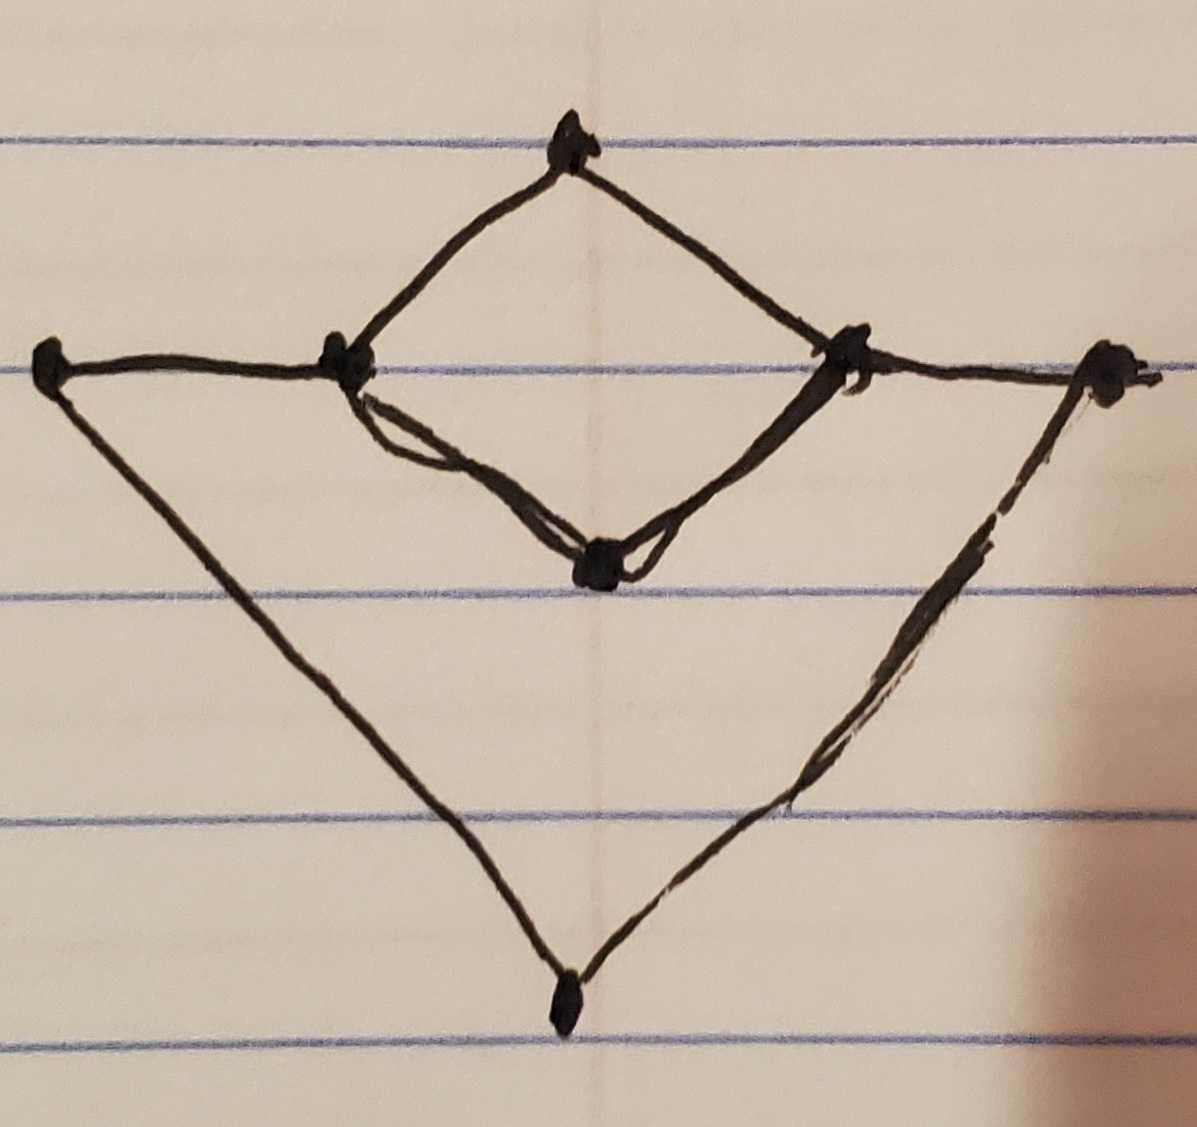
\includegraphics[width = 7cm]{problem4}\\
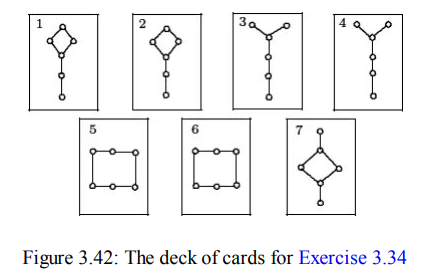
\includegraphics[width=7cm]{fig342}


\end{document} 




















